%!TEX root = lec05_query_processing.tex


%
% --------------------------------------------------------------------------------------------------------------------------------------
%
\begin{frame}[fragile]{Compiling SQL into algebra expressions}

Recap: 

\begin{itemize}[-]
\item SQL is a complex language, with many sophisticated constructs that are beyond our scope here. Instead we focus on the basic building blocks.

\item \alert{A query plan is, essentially, an algebra expression} with access methods instead of table names.

\item The main difference between a plan and a ``pure'' algebra expression is that in the plan we need to specify the access methods we use to read the database.
\end{itemize}

\end{frame}


\newsavebox\algebraBasicSelectFromWhere
\savebox{\algebraBasicSelectFromWhere}{
    \begin{tikzpicture}[align=center,node distance=0.825cm,every node/.style={inner sep=1,outer sep=1,font=\footnotesize}]
    \node (P1) at (0,0) {$\pi_{a_1,\ldots,a_n}$};
    \node (P2) [below of=P1] {$\sigma_{c_1\ \wedge\ \cdots\ \wedge c_k}$};
    \node (P3) [below of=P2] {$\times$};
    \node (P4) [below left=0.25cm and 0.25cm of P3] {$\times$};
    \node (P5) [below right=0.25cm and 0.25cm of P3] {$T_m$};
    \node (P6) [below right=0.25cm and 0.25cm of P4] {$T_{m-1}$};
    \node (P7) [inner sep=4,below left=0.25cm and 0.125cm of P4] {$\cdots$};
    \node (P8) [below left=0.25cm and 0.125cm of P7] {$\times$};
    \node (P9) [below left=0.25cm and 0.125cm of P8] {$T_1$};
    \node (P10) [below right=0.25cm and 0.125cm of P8] {$T_2$};
    \path[commutative diagrams/.cd, every arrow]
        (P2) edge (P1)
        (P3) edge (P2)
        (P4) edge (P3)
        (P5) edge (P3)
        (P6) edge (P4)
        (P7) edge (P4)
        (P8) edge (P7)
        (P9) edge (P8)
        (P10) edge (P8);
\end{tikzpicture}%
}

%
% --------------------------------------------------------------------------------------------------------------------------------------
%
\begin{frame}[fragile]{Compiling basic SQL expressions}

\begin{columns}[onlytextwidth]
\begin{column}{0.5\textwidth}

The basic compilation step translates a \textbf{conjunctive SQL query} into a ``\alert{\textbf{canonical}}'' plan like:

\vskip1em

\begin{lstlisting}[style=SQL,escapeinside={(*}{*)},frame=single]
SELECT (*$a_1, a_2, \ldots, a_n$*)
FROM (*$T_1$*) [, (*$T_2$*) [, (*$\ldots$*) [, (*$T_m$*)]]]
WHERE (*$c_1$*) AND (*$c_2$*) AND (*\ldots*) AND (*$c_k$*)
\end{lstlisting}
\end{column}

\vspace*{-2.5em}
\begin{column}{0.45\textwidth}
\usebox\algebraBasicSelectFromWhere
\end{column}
\end{columns}

\vskip2em

If there is a single table expression\\ in the query, we omit the Cartesian product of course.

We omit the \lstinline[style=SQL]{scan()} operators here for simplicity.

\end{frame}


%
% --------------------------------------------------------------------------------------------------------------------------------------
%
\begin{frame}[fragile]

The \alert{\emph{renaming operator} $\rho()$} is used to handle the tuple variable declarations in SQL.


\vskip3em

\begin{columns}
\begin{column}{0.5\textwidth}
\begin{lstlisting}[style=SQL,frame=single]
SELECT m.title, m.year
FROM Movie -:m:-
WHERE m.director = 'Ivan Reitman'
\end{lstlisting}
\end{column}
\begin{column}{0.4\textwidth}
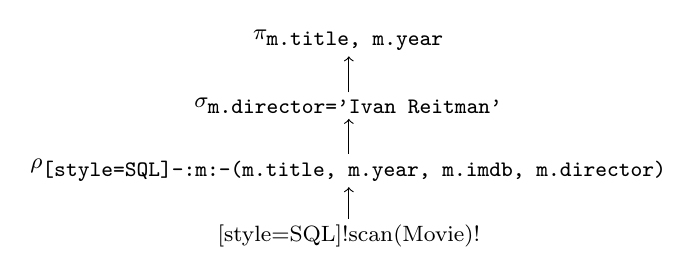
\begin{tikzpicture}[align=center,node distance=0.825cm,every node/.style={inner sep=1,outer sep=1,font=\footnotesize}]
\node (pi) at (0,0) {$\pi_{\texttt{m.title, m.year}}$};
\node (sigma) [below of=pi] {$\sigma_{\texttt{m.director='Ivan Reitman'}}$};
\node (rho) [below of=sigma] {$\rho_{\texttt{\lstinline[style=SQL]{-:m:-}(m.title, m.year, m.imdb, m.director)}}$};
\node (Movie) [below of=rho] {\lstinline[style=SQL]!scan(Movie)!};
\path[->]
	(Movie) edge (rho)
	(rho) edge (sigma)
	(sigma) edge (pi);
\end{tikzpicture}
\end{column}
\end{columns}
\end{frame}

%
% --------------------------------------------------------------------------------------------------------------------------------------
%

\newsavebox\bmmMovieCrossProduct
\savebox{\bmmMovieCrossProduct}{
    \begin{tikzpicture}[align=center,node distance=0.825cm,every node/.style={inner sep=1,outer sep=1,font=\footnotesize}]
    \node (P1) at (0,0) {$\pi_{\texttt{m.director}}$};
    \node (P2) [below of=P1] {$\sigma_{\substack{\texttt{m.year=bmm.year}\\\wedge\ \texttt{m.title=bmm.title}}}$};
    \node (P3) [below of=P2] {$\times$};
    \node (P4) [below of=P3,xshift=1.5cm] {$\rho_{\substack{\texttt{bmm(bmm.title,}\\%
           \texttt{bmm.year)}}}$};
    \node (P5) [below of=P3,xshift=-1cm] {$\rho_{\substack{\texttt{m(m.title, m.year}\\
           \texttt{m.imdb,m.director)}}}$};
    \node (P6) [below=0.5cm of P4] {$\pi_{\texttt{title,year}}$};           
    \node (P7) [below=0.5cm of P6] {$\sigma_{\texttt{actor='Bill Murray'}}$};
    \node (P8) [below=0.5cm of P7] {\lstinline[style=SQL]!scan(Cast)!};
    \node (P9) [below=0.5cm of P5] {\lstinline[style=SQL]!scan(Movie)!};
    \path[commutative diagrams/.cd, every arrow]
        (P2) edge (P1)
        (P3) edge (P2)
        (P4) edge (P3)
        (P5) edge (P3)
        (P6) edge (P4)
        (P7) edge (P6)
        (P8) edge (P7)
        (P9) edge (P5);
\end{tikzpicture}}


\newsavebox\bmmMovieJoin
\savebox{\bmmMovieJoin}{
    \begin{tikzpicture}[align=center,node distance=0.825cm,every node/.style={inner sep=1,outer sep=1,font=\footnotesize}]
    \node (P1) at (0,0) {$\pi_{\texttt{m.director}}$};
    \node (P3) [below of=P1] {$\Join_{\substack{\texttt{m.year=bmm.year}\\\wedge\ \texttt{m.title=bmm.title}}}$};
    \node (P4) [below of=P3,xshift=1.5cm] {$\rho_{\substack{\texttt{bmm(bmm.title,}\\%
           \texttt{bmm.year)}}}$};
    \node (P5) [below of=P3,xshift=-1cm] {$\rho_{\substack{\texttt{m(m.title, m.year}\\
           \texttt{m.imdb,m.director)}}}$};
    \node (P6) [below=0.5cm of P4] {$\pi_{\texttt{title,year}}$};           
    \node (P7) [below=0.5cm of P6] {$\sigma_{\texttt{actor='Bill Murray'}}$};
    \node (P8) [below=0.5cm of P7] {\lstinline[style=SQL]!scan(Cast)!};
    \node (P9) [below=0.5cm of P5] {\lstinline[style=SQL]!scan(Movie)!};
    \path[commutative diagrams/.cd, every arrow]
        (P3) edge (P1)
        (P4) edge (P3)
        (P5) edge (P3)
        (P6) edge (P4)
        (P7) edge (P6)
        (P8) edge (P7)
        (P9) edge (P5);
\end{tikzpicture}}

\begin{frame}[fragile]

Table expressions given as SQL queries are translated into \textbf{sub-expressions} ``below the Cartesian product'' in the main plan:

\vskip2em

\begin{columns}
\begin{column}{0.425\textwidth}
\begin{lstlisting}[style=SQL,frame=single]
SELECT m.director
FROM Movie m, 
  (SELECT title, year 
   FROM Cast
   WHERE actor='Bill Murray'
  ) AS bmm
WHERE m.year=bmm.year 
  AND m.title=bmm.title;
\end{lstlisting}
\end{column}
\begin{column}{0.4\textwidth}
% \vspace*{-2em}
\usebox{\bmmMovieCrossProduct}
\end{column}
\end{columns}
\end{frame}

%
% --------------------------------------------------------------------------------------------------------------------------------------
%
\begin{frame}

It is OK to ``\textbf{\alert{push down}}'' conditions in the \lstinline[style=SQL]{WHERE} clause that define a join, replacing the Cartesian product when possible:


\vskip2em

\begin{columns}
\begin{column}{0.425\textwidth}
\scalebox{0.9}{\usebox{\bmmMovieCrossProduct}}
\end{column}
\begin{column}{0.4\textwidth}
\usebox{\bmmMovieJoin}
\end{column}
\end{columns}


\end{frame}


%
% --------------------------------------------------------------------------------------------------------------------------------------
%
\begin{frame}[fragile]

Set/bag operators are also translated into their algebra counterparts:

\textbf{Example:}

\begin{columns}
\begin{column}{0.425\textwidth}
\begin{lstlisting}[style=SQL,frame=single]
SELECT title, year
FROM Cast
WHERE actor="Bill Murray"
INTERSECT
SELECT title, year 
FROM Movie
WHERE imdb>7
\end{lstlisting}
\end{column}
\begin{column}{0.4\textwidth}
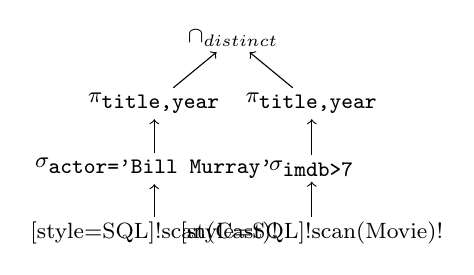
\begin{tikzpicture}[align=center,node distance=0.825cm,every node/.style={inner sep=1,outer sep=1,font=\footnotesize}]
    \node (intersection) at (0,0) {$\cap_{\text{distinct}}$};
    \node (sub1) [below of=intersection,xshift=-1cm] {$\pi_{\texttt{title,year}}$};
    \node (sub2) [below of=intersection,xshift=1cm] {$\pi_{\texttt{title,year}}$};
    \node (sigma1) [below of=sub1] {$\sigma_{\texttt{actor='Bill Murray'}}$};
    \node (Cast) [below of=sigma1] {\lstinline[style=SQL]!scan(Cast)!};
    \node (sigma2) [below of=sub2] {$\sigma_{\texttt{imdb>7}}$};
    \node (Movie) [below of=sigma2] {\lstinline[style=SQL]!scan(Movie)!};
    \path[->]
        (Cast) edge (sigma1)
        (sigma1) edge (sub1)
        (sub1) edge (intersection)
        (Movie) edge (sigma2)
        (sigma2) edge (sub2)
        (sub2) edge (intersection);
\end{tikzpicture}
\end{column}
\end{columns}
\end{frame}


%
% --------------------------------------------------------------------------------------------------------------------------------------
%
\begin{frame}[fragile]
Aggregation is handled by operator \(\gamma_{\text{<grouping>,fn()}}(R)\)

\vskip0.5em

The \lstinline[style=SQL]{GROUP BY} clause goes into ``grouping'' and \lstinline[style=SQL]{fn()} is the set function. The \lstinline[style=SQL]{HAVING} clause are handled with a selection.

\vskip2em

\begin{columns}
\begin{column}{0.4\textwidth}
\begin{lstlisting}[style=SQL,frame=single]
SELECT theater, COUNT(*) 
FROM Guide
WHERE start > 1100
GROUP BY theater
HAVING COUNT(*) > 4
\end{lstlisting}
\end{column}
\begin{column}{0.3\textwidth}
\scalebox{1}{
     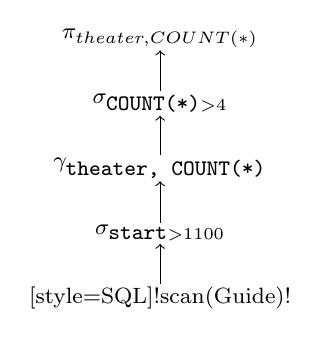
\begin{tikzpicture}[align=center,node distance=0.825cm,every node/.style={inner sep=0.5,outer sep=0.5,font=\footnotesize}]
    \node (P1) at (0,0) {$\pi_{\text{theater, COUNT(*)}}$};
    \node (P2) [below of=P1] {$\sigma_{\texttt{COUNT(*)}>4}$};
    \node (P3) [below of=P2] {$\gamma_{\texttt{theater, COUNT(*)}}$};
    \node (P4) [below of=P3] {$\sigma_{\texttt{start}>1100}$};
    \node (P5) [below of=P4] {\lstinline[style=SQL]!scan(Guide)!};
    \path[->]
        (P2) edge (P1)
        (P3) edge (P2)
        (P4) edge (P3)
        (P5) edge (P4);
\end{tikzpicture}%
}
\end{column}
\end{columns}
\end{frame}


%
% --------------------------------------------------------------------------------------------------------------------------------------
%
\begin{frame}[fragile]{Sub-Queries in Other Expressions}

Recall SQL allows sub-queries to appear inside value expressions and in predicates in the \lstinline[style=SQL]{WHERE} clause.

\vskip2em

\begin{columns}[onlytextwidth]
\begin{column}{0.4\textwidth}
\begin{lstlisting}[style=SQL]
SELECT 100 + (
        SELECT COUNT(*)
        FROM Movie
       );
\end{lstlisting}
\end{column}
\begin{column}{0.5\textwidth}
\begin{lstlisting}[style=SQL]
SELECT m.title 
FROM Movie m
WHERE m.imdb = (SELECT MAX(imdb)
                FROM Movie);
\end{lstlisting}
\end{column}
\end{columns}

\vskip2em


Actual query plans in production DBMSs have nodes beyond the relational algebra (e.g., to handle complex arithmetic or string operations from the results of sub-queries).
\end{frame}

\newsavebox{\preprocessorCTEexample}
\begin{lrbox}{\preprocessorCTEexample}
\begin{minipage}{0.5\textwidth}
\begin{lstlisting}[style=SQL]
WITH TopMovie(title, year) AS (
    SELECT title, year 
    FROM Movie WHERE imdb > 7
)
SELECT c.role
FROM Cast c, TopMovie tm
WHERE c.title=tm.title AND 
      c.year=tm.year AND
      c.actor="Sigourney Weaver";
\end{lstlisting}
\end{minipage}
\end{lrbox}

\newsavebox{\preprocessorCTEexampleRewritten}
\begin{lrbox}{\preprocessorCTEexampleRewritten}
\begin{minipage}{0.5\textwidth}
\begin{lstlisting}[style=SQL,escapechar=|]
SELECT c.role
FROM Cast c, |\alert{(}|
    |\alert{SELECT title, year}| 
    |\alert{FROM Movie WHERE imdb > 7}|
    |\alert{) AS tm}|
WHERE c.title=tm.title AND 
      c.year=tm.year AND
      c.actor="Sigourney Weaver";
\end{lstlisting}
\end{minipage}
\end{lrbox}

%
% --------------------------------------------------------------------------------------------------------------------------------------
%
\begin{frame}[fragile]{The SQL Preprocessor}

Other constructs in SQL such as \emph{views} and Common Table Expressions (CTEs) given through \lstinline[style=SQL]{WITH} clauses are handled by the SQL \textbf{preprocessor}.

Views and non-recursive CTEs are treated essentially as \emph{macros} in a C program: the preprocessor replaces every occurrence of the CTE or the view in a table expression by that CTE/view definition:

\vskip1em

\begin{columns}
\begin{column}{0.4\textwidth}
\scalebox{0.75}{\usebox\preprocessorCTEexample}
\end{column}
\begin{column}{0.4\textwidth}
\scalebox{0.75}{\usebox\preprocessorCTEexampleRewritten}
\end{column}
\end{columns}
\end{frame}
